\hypertarget{xmlparse_8inc}{
\section{include/xmlparse.inc File Reference}
\label{xmlparse_8inc}\index{include/xmlparse.inc@{include/xmlparse.inc}}
}
Functions to parse \hyperlink{classXML}{XML} data. 

\subsection*{Functions}
\begin{CompactItemize}
\item 
\hyperlink{xmlparse_8inc_2ee17c038e8fe8a1ddc86bb533863cb7}{parseXML} (\$url)
\end{CompactItemize}


\subsection{Detailed Description}
Functions to parse \hyperlink{classXML}{XML} data. 

Functions to parse \hyperlink{classXML}{XML} data. Specifaclly created for use with isbndb.com 

Definition in file \hyperlink{xmlparse_8inc-source}{xmlparse.inc}.

\subsection{Function Documentation}
\hypertarget{xmlparse_8inc_2ee17c038e8fe8a1ddc86bb533863cb7}{
\index{xmlparse.inc@{xmlparse.inc}!parseXML@{parseXML}}
\index{parseXML@{parseXML}!xmlparse.inc@{xmlparse.inc}}
\subsubsection{\setlength{\rightskip}{0pt plus 5cm}parseXML (\$ {\em url})}}
\label{xmlparse_8inc_2ee17c038e8fe8a1ddc86bb533863cb7}


Parse \hyperlink{classXML}{XML} Data from the given URL \begin{Desc}
\item[Parameters:]
\begin{description}
\item[{\em \$url}]Location of \hyperlink{classXML}{XML} data \end{description}
\end{Desc}
\begin{Desc}
\item[Returns:]Object containing parsed \hyperlink{classXML}{XML} data \end{Desc}


Definition at line 15 of file xmlparse.inc.

References fget().

Referenced by getBarcodeInfo().

\begin{Code}\begin{verbatim}15                         {
19   $xmlstr = fget($url);
23   $xml = new SimpleXMLElement($xmlstr);
24 
25   return $xml;
26 }\end{verbatim}
\end{Code}




Here is the call graph for this function:\nopagebreak
\begin{figure}[H]
\begin{center}
\leavevmode
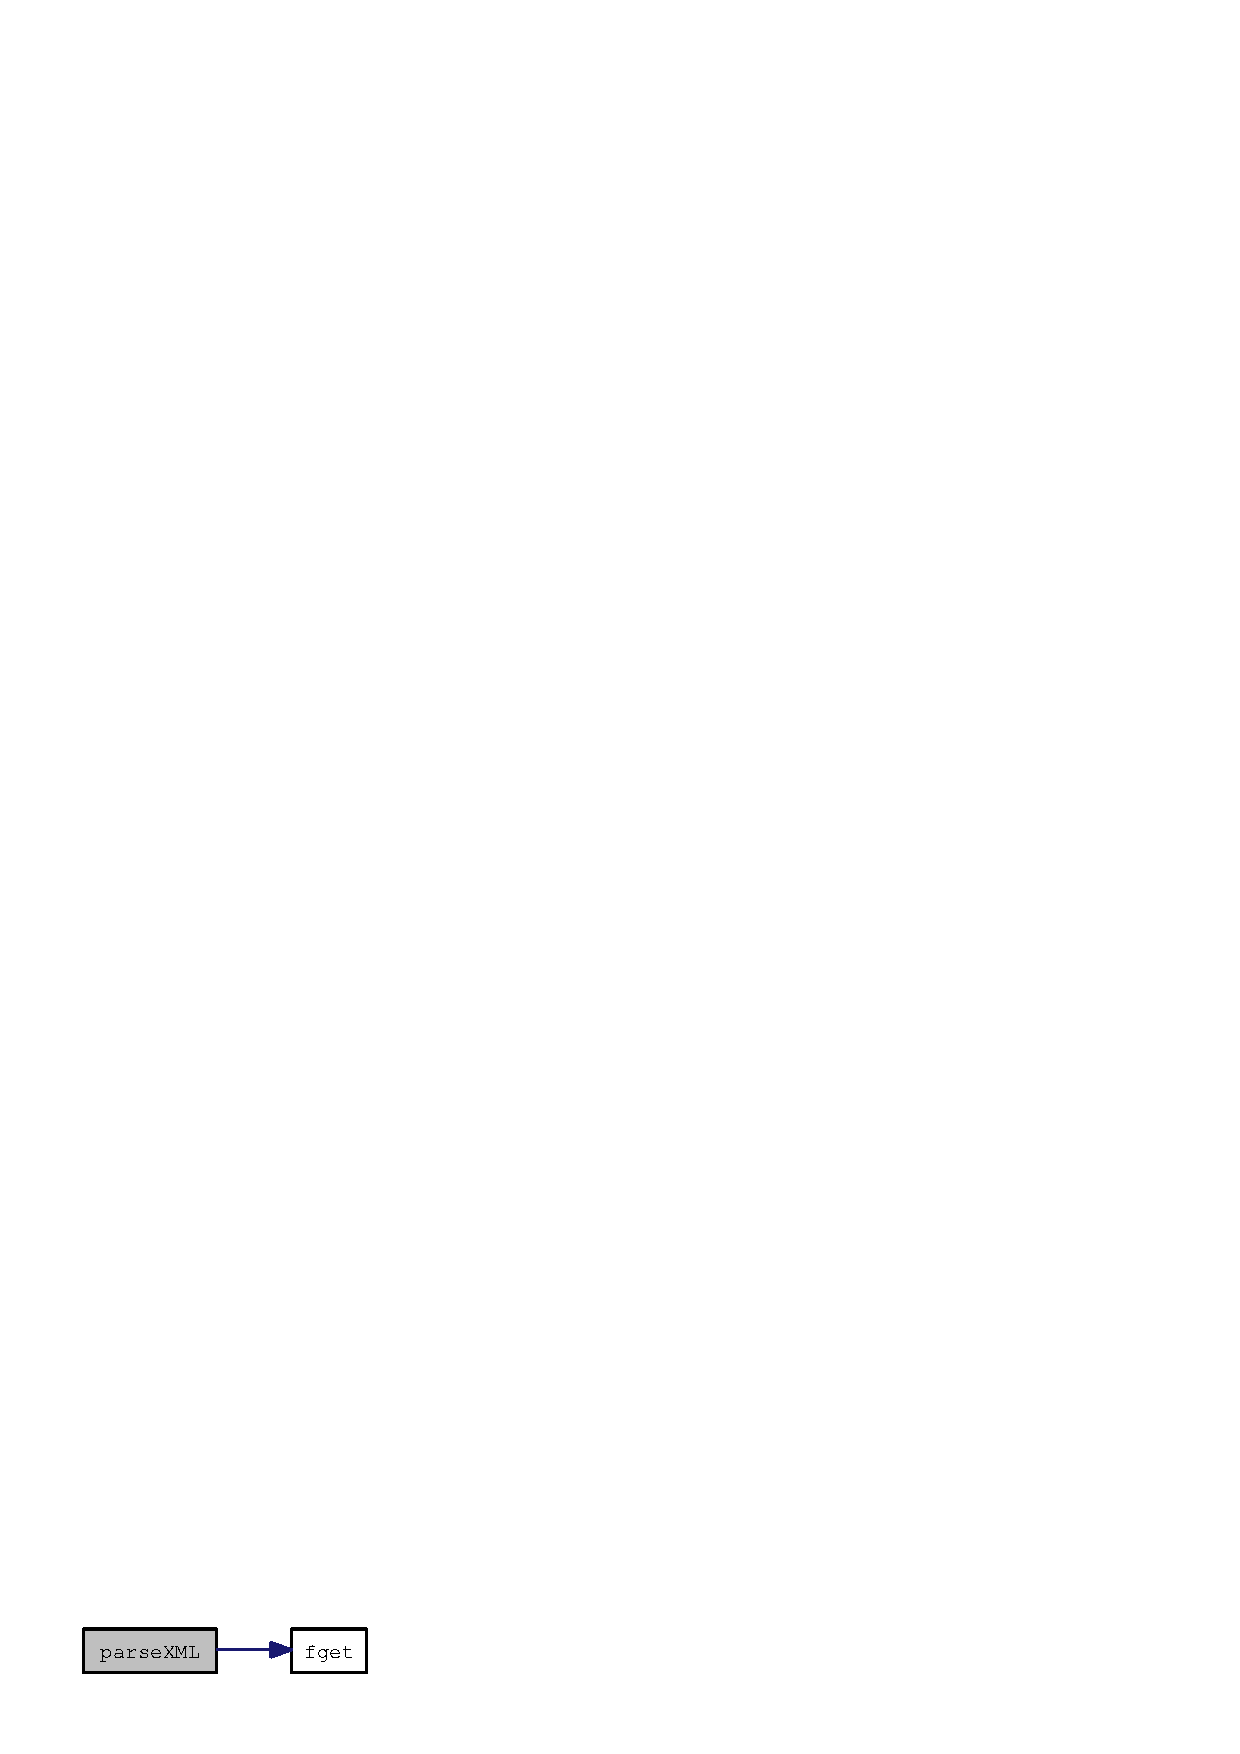
\includegraphics[width=90pt]{xmlparse_8inc_2ee17c038e8fe8a1ddc86bb533863cb7_cgraph}
\end{center}
\end{figure}


Here is the caller graph for this function:\nopagebreak
\begin{figure}[H]
\begin{center}
\leavevmode
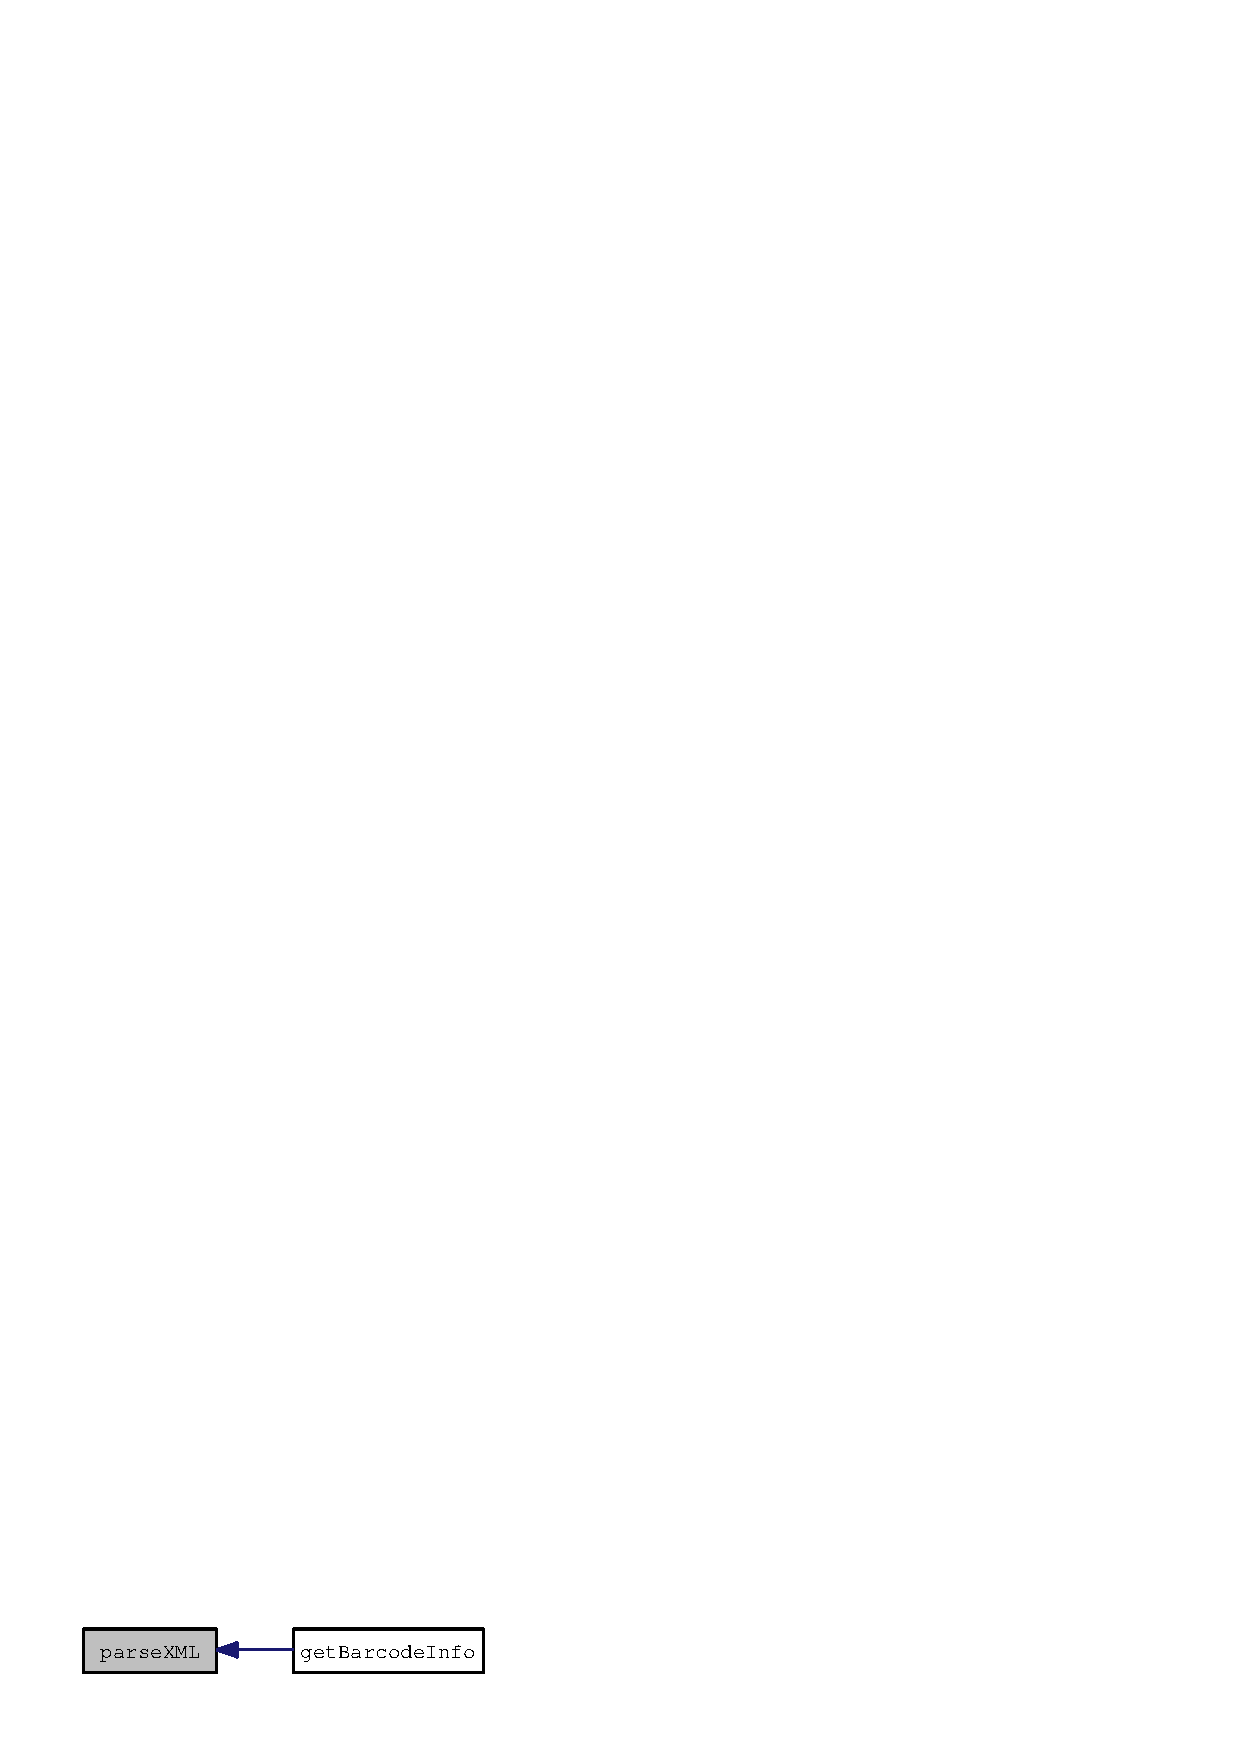
\includegraphics[width=118pt]{xmlparse_8inc_2ee17c038e8fe8a1ddc86bb533863cb7_icgraph}
\end{center}
\end{figure}
